
What follows are instructions for interacting with the Galant GUI interface.

\subsection{Overview}

Galant provides three major components across two windows:
\begin{enumerate}
\item
a text window that can serve two distinct purposes --
\begin{enumerate}
\item as an editor of algorithms
\item as an editor of GraphML representations of graphs
\end{enumerate}
\item
a graph window that displays the current graph (independent of whether
the text window shows an algorithm or the GraphML representation of the graph)
\end{enumerate}

It is usually more convenient to edit algorithms
offline using a program editor.
The primary use of the text editor is to correct minor errors and
to see the syntax highlighting related to macros and Galant API functions.
The graph window is the primary mechanism for editing graphs.
One exception is when precise adjustments node positions are desired.
Weights and labels are sometimes also easier to edit in the text window.

\begin{figure*}
  \centering
    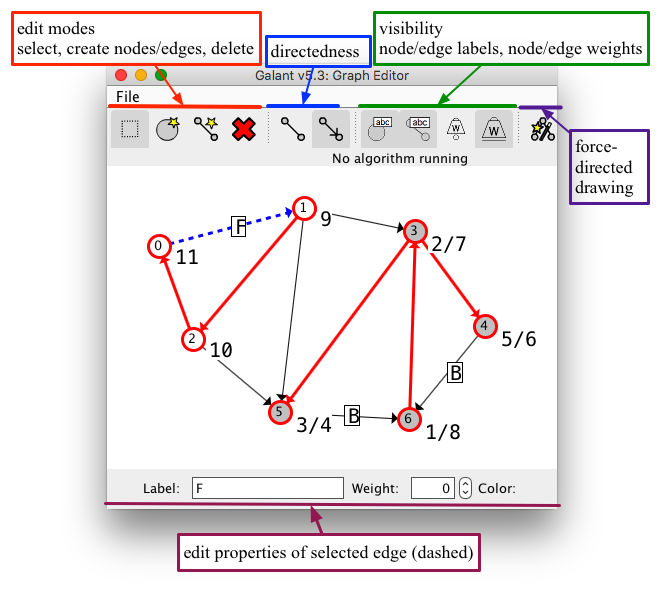
\includegraphics[scale=0.5]{X-graph_window-annotated}

    Graph window: add/delete nodes and edges, move nodes, etc.

    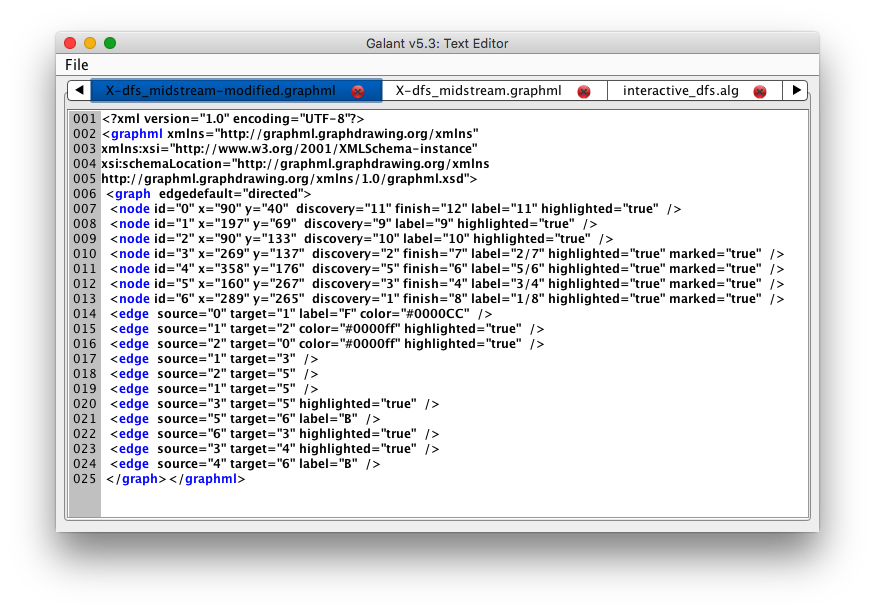
\includegraphics[scale=0.5]{X-dfs_midstream_modified-text}

    \vspace{-3ex}
    Text window: GraphML representation.

  \caption{The Galant user interface.}
  \label{fig:user_interface}
\end{figure*}

% [Last modified: 2016 12 13 at 21:24:38 GMT]


These components operate in two modes: edit mode and animation mode.
Edit mode allows the user to modify graphs -- see Sec.~\ref{sec:graph_editing},
or algorithms -- see Sec.~\ref{sec:algorithm_editing}. Animation mode disables all forms of modification, allowing the user to progress through
an animation by stepping forward or backward, as described in
Sec.~\ref{sec:animating_algorithms}.

\subsection{Workspace}

Opened graph and algorithm files are displayed in the text window,
which has tabs that allow the user to switch among different algorithms/graphs.
New algorithms are created using the icon that looks like
a page of text at the top left of the
window; new graphs are created
using the graph/tree icon to the left of that.
More commonly, algorithm and graph files are loaded via the \Code{File->Open}
browser dialog. The \Code{File} drop-down menu also allows saving of files
and editing of preferences. Algorithm files have the extension \Code{.alg}
and graph files the extension \Code{.graphml}.

Fig.~\ref{fig:user_interface} shows both the graph window (top) and the text
window (bottom). Annotations on the graph window describe the components of
the window that can be used to edit a graph visually.

\subsection{Graph editing}
\label{sec:graph_editing}

Graphs can be edited in their GraphML representation using the text window
or visually using the graph window.
These editors are linked:
any change in the visual representation is immediately reflected in the text
representation (and will overwrite what was originally there);
a change in the GraphML representation will take effect in the visual representation
when the file is saved.

An improperly formatted GraphML file loaded from an external source will
result in an error.
Galant reports errors of all kinds (during reading of files, compilation of
animation programs or execution of animations)
by displaying a pop up window that allows the user to choose whether to
continue (and usually return to a stable state) or quit the program.
Error information, including a stack trace, is also displayed on the console.

The graph window, as illustrated at the top of Fig.~\ref{fig:user_interface},
has a toolbar with four sections:
\begin{enumerate}
\item
\textbf{Graph edit mode -- }
this includes the \emph{select}, \emph{create node}, \emph{create edge}, and \emph{delete} buttons.
Only one button is active at any time; it determines the effect
of a user's interaction (mouse clicking, dragging, etc.) with the window.
if there are conflicts in selection of objects, nodes with higher id numbers have precedence (are above those with lower id numbers) and nodes
have precedence over edges (are above edges).
\begin{itemize}
\item \emph{Select.} A mouse click selects the graph component with highest precedence.
If the component is a node, it is shaded light blue; if it's an edge, it
becomes dashed.
The in-line editor at the bottom of the graph window allows editing of the
component's label, weight, and color.
\item \emph{Create node.}
A node is created at the location of a mouse click if there is not already a node there.
If another node is present it is simply selected.
\item \emph{Create edge.}
Two clicks are required to create an edge. The first falls on the desired
source node and the second on the target node.
The line representing the edge is shown after the first click.
If the first click does not land on a node, no edge is created.
If the second click does not land on a node, creation of the edge is canceled.
\item \emph{Delete.}
A mouse click deletes the highest-precedence component at the mouse location.
If a node is deleted, all of its incident edges are deleted as well.
\end{itemize}

\item
\textbf{Directedness toggles --}
These change both the interpretation and the
display of the graph between directed and undirected.
Pressing the undirected (line without arrows) button causes
all edges to be interpreted as undirected: this means that, when the code
calls for all incoming/outgoing edges, all incident edges are used.
Undirected edges are displayed as simple lines.

Pressing the directed (line with arrow) button causes the macros
\Code{for\_incoming}, \Code{for\_outgoing}, and \Code{for\_adjacent}
to have three distinct meanings (they are all the same for undirected graphs):
Incoming edges have the given node as target, outgoing as source, and adjacent applies to all incident edges.

\item
\textbf{Display toggles --}
The four display toggles turn on/off the display of node/edge labels and node/edge weights.
A shaded toggle indicates that the corresponding display is \emph{on}.
When Galant is executed for the first time, all of these are \emph{on},
but their setting persists from session to session.
Labels and weights are also all displayed at the beginning of execution of
an animation.
The animation program can choose to hide labels and/or weights with simple
directives.
Hiding is usually unnecessary -- the graphs that are subjects of the animations
typically have only the desired attributes set.

\item
\textbf{Force directed drawing button -- }
Applies Hu's force directed algorithm~\cite{2006-Mathematica-Hu} to the graph.
Pushing the button a second time causes the drawing to revert to its previous state.
Fig.~\ref{fig:force_directed} illustrates the use of force directed drawing
to massage a randomly generated graph for convenient use in animations.
The graph was generated randomly as a list of edges with weights
and converted to graphml using a simple script.
Galant, when reading the graph initially, assigned random positions to the nodes.

\end{enumerate}

\begin{figure*}
  \begin{center}

    \hspace*{-4em}
    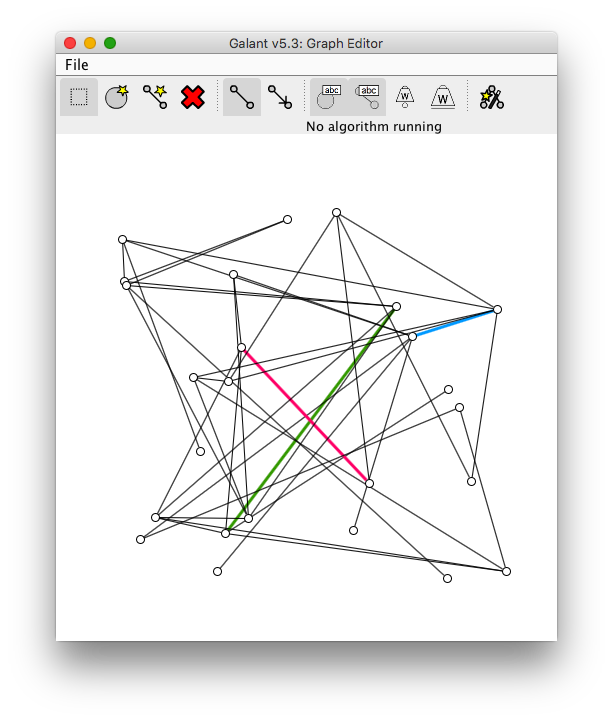
\includegraphics[width=0.375\textwidth]{X-r_25_40_1}
    \hspace{-2em}
    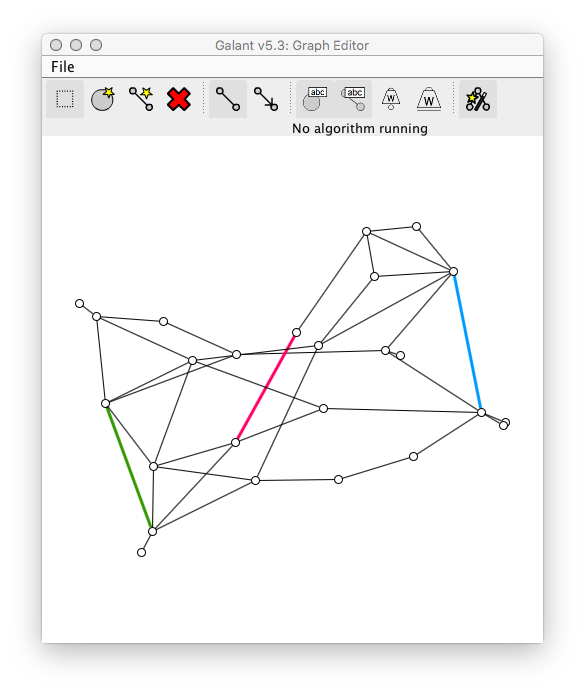
\includegraphics[width=0.375\textwidth]{X-r_25_40_1-fd}
    \hspace{-2em}
    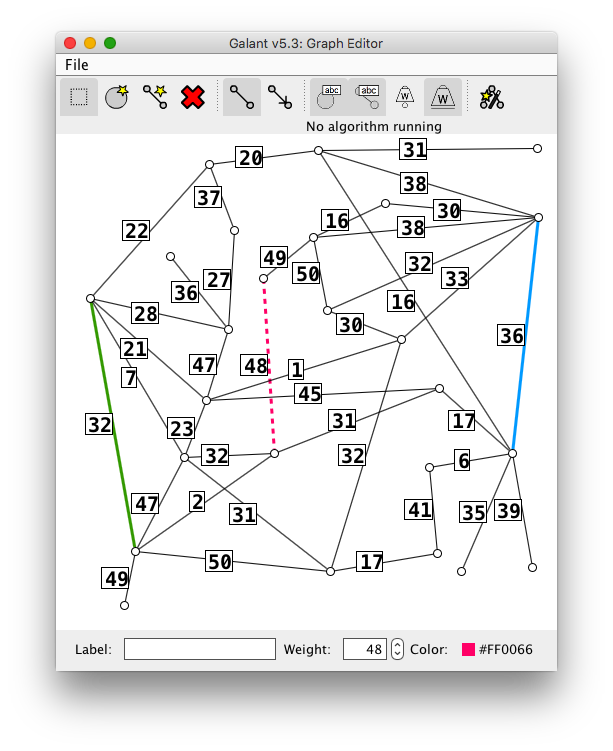
\includegraphics[width=0.375\textwidth]{X-r_25_40_1-edited}

    \hspace*{-4em}
    \parbox[c][3ex][c]{0.35\textwidth}{
      (a) A graph from an external random generator.
    }
%    \hspace{-2em}
    \parbox[c][3ex][c]{0.35\textwidth}{
    (b) Force directed layout applied.
    }
%    \hspace{-2em}
    \parbox[c][3ex][c]{0.35\textwidth}{
    (c) User moved nodes for an even better layout.
    }

  \end{center}

  \bigskip
  \caption{Using force directed drawing to lay out graphs for more convenient
    editing and more compelling animations. Node ids do not appear because
    a node radius of~3 was specified using the
    \Code{Preferences$\rightarrow$Graph~Display} panel.}

  \label{fig:force_directed}
\end{figure*}

% [Last modified: 2017 01 06 at 01:42:15 GMT]


Keyboard shortcuts for graph editing operations are as follows:

\begin{tabular}{l @{ -- } p{0.9\textwidth}}
\textsf{Ctrl-n} & create a new node in a random position \\
\textsf{Ctrl-e} & create a new edge; user is prompted for id's of the nodes to
be connected \\
\textsf{Ctrl-i} & do a smart repositioning (force-directed)
of nodes of the graph, useful when positions were chosen randomly
\\
\textsf{Del-n} & (hold delete key when typing \Code{n})
delete a node; user is prompted for id \\
\textsf{Del-e} & delete an edge; user is prompted for id's of the endpoints \\
\textsf{Ctrl-$\ell$} & toggle display of node labels \\
\textsf{Ctrl-L} & toggle display of edge labels \\
\textsf{Ctrl-w} & toggle display of node weights \\
\textsf{Ctrl-W} & toggle display of edge weights \\
\end{tabular}

\subsection{Algorithm editing}
\label{sec:algorithm_editing}

Algorithms can be edited in the text window. The
editor uses Java keyword highlighting (default blue) and
highlighting of Galant API fields and methods (default green).
Since the current algorithm editor is fairly primitive (no search and replace, for example),
it is more efficient to edit animation code offline using a program editor --
for example \Code{emacs} with Java mode turned on.
The Galant editor is, however, useful for locating and correcting minor errors.
For more details on how to compose animation code, see the programmer guide
(Section~\ref{sec:programmer_guide}).

\subsection{Animating algorithms}
\label{sec:animating_algorithms}

\begin{figure}
  \begin{center}
  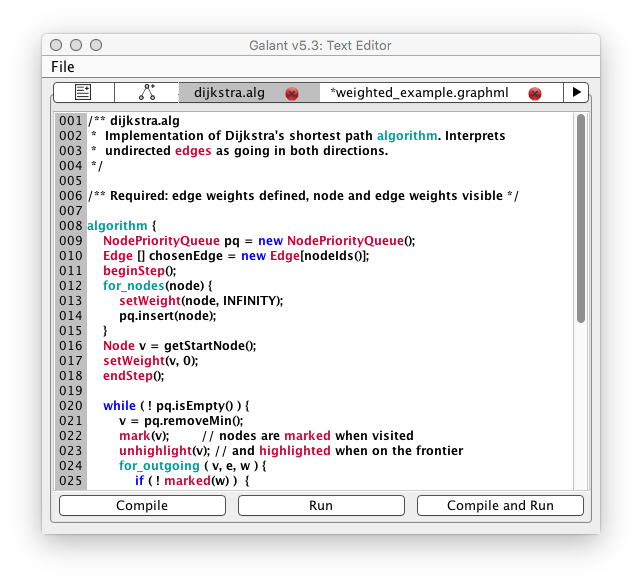
\includegraphics[scale=0.45]{X-dijkstra_text}

  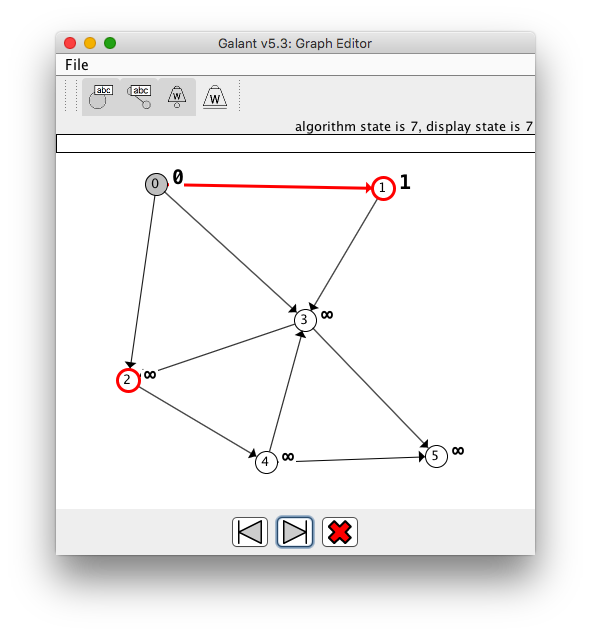
\includegraphics[scale=0.45]{X-dijkstra_running}
  \end{center}

  \caption{The text and graph windows when an algorithm is running. The text
    window is at the top -- it has buttons for the user to select
    whether to compile the algorithm, run it (if already compiled) or do
    both. The graph window in the middle of algorithm execution is at
    the bottom.}
  \label{fig:dijkstra_running}
\end{figure}

% [Last modified: 2016 12 22 at 22:25:28 GMT]


To animate an algorithm the code for it must be compiled and then run via the
algorithm controls
 -- the bottom tabs on the text window shown in Fig.~\ref{fig:dijkstra_running}.
The algorithm runs on the \emph{active graph}, the one currently displayed
on the graph window, also shown in Fig.~\ref{fig:dijkstra_running}.
While the algorithm is running, its text is grayed out.\footnote{
  This may not be desirable. The intent was to indicate to the user that
  operations on the text window are not desired.
  }
If there are errors in compilation these will show up on the console (terminal
from which Galant was run) and in a dialog box that allows the user to ask for more details
and decide whether to exit Galant or not.
The console also displays the what the code looks like after macro replacement
in case obscure errors were the result of unexpected macro expansion.
Line numbers in the macro-expanded code match those of the original so that
all errors reported by the Java compiler will refer to the correct line number
in the original Galant code.
Runtime errors also open the above mentioned
dialog box.

When the user initiates execution of an animation by pushing the \textsf{Run}
button
the animation program
steps forward until
displays the next animation event or, if a \Code{beginStep()}
call has marked the start of a sequence of events, until
it reaches the next \Code{endStep()} call.
It then pauses execution and waits for the user to decide whether to
step forward, step backward, or exit.
A step forward resumes execution while a step backward returns the display to a previous
state.
The algorithm resumes execution only when the \emph{display state}
indicated by the user's sequence of forward and backward steps
($f-b$, where $f$ is the number of forward and $b$ the number of backward steps)
exceeds the \emph{algorithm state}, the number of animation steps the algorithm
has executed.
The user controls forward and backward steps using either the buttons at the
bottom of the graph window (shown in Fig.~\ref{fig:dijkstra_running})
or the right/left arrow keys.
During the execution of the animation, all graph editing functions are disabled.
These are re-enabled when the user exits the animation by pressing the red \textbf{X} button or the \textsf{Esc} (escape) key on the terminal.

\subsection{Preferences}
\label{sec:preferences}

Galant preferences can be accessed via the \Code{File->Preferences}
menu item or by using the keyboard shortcut \textsf{Ctrl-P}
(\textsf{Cmd-P} for Mac).
Preferences that can be edited are:
\begin{itemize}
\item
Default directories for opening and saving files (\Code{Open/Save}).
\item
Directory where compiled animation code is stored (\Code{Compilation}).
\item
Font size and tab size for text window editing (\Code{Editors}).
\item
Colors for keyword and Galant API highlighting (\Code{Algorithm~Editor}).
\item
Color for GraphML highlighting (\Code{Textual~Graph~Editor}).
\item
Node radius (\Code{Graph~Display});
when the radius is below a threshold (9 pixels), node id's are not displayed;
this is useful when running animations on large graphs.
\item
Edge width (\Code{Graph~Display}).
\end{itemize}

\begin{figure}
  \centering

  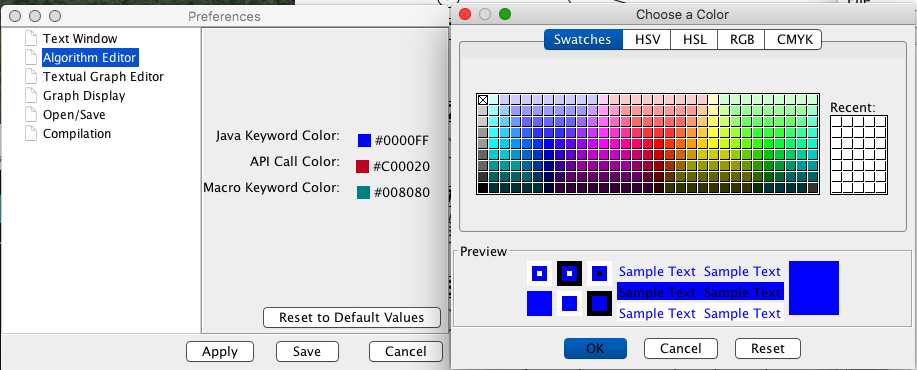
\includegraphics[scale=0.45]{X-syntax_highlight_preference}

  (a) syntax highlight colors -- same color chooser as for editing node/edge
  colors

  \medskip
  \parbox{\textwidth}{
    \hspace*{-2em}
    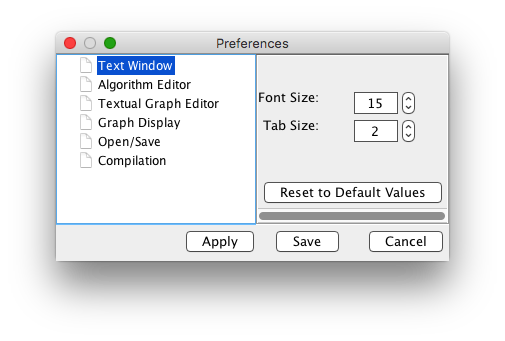
\includegraphics[scale=0.45]{X-text_preference}
    \hspace{-3em}
    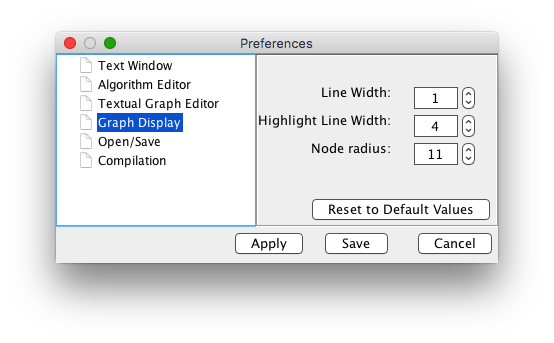
\includegraphics[scale=0.45]{X-graph_display_preference}
  }

  \vspace{-5ex}

  \hspace*{-2em}
  (b) text font size and tab spaces
  \hspace{3em}
  (c) line widths and node radius

  \medskip
  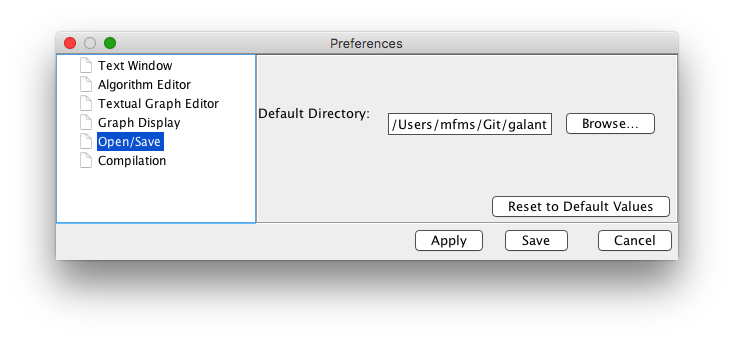
\includegraphics[scale=0.5]{X-directory_preference}

  \vspace{-5ex}
  (d) default directory for opening and saving files

  \caption{The four most important preference panels.}
  \label{fig:preference_panels}
\end{figure}

% [Last modified: 2017 01 06 at 14:02:15 GMT]


Fig.~\ref{fig:preference_panels} shows the four preference panels of most
interest to the user.

% [Last modified: 2017 01 06 at 13:47:38 GMT]
